\chapter{Fast One-Ring Smoothing Filtering}
The Fast One-Ring smoothing filter was initially proposed by H. Mara and S. Krömker at the EUROGRAPHICS Workshop on Graphics and Cultural Heritage (2017) ~\cite[s.~3.2]{Mara17}. Further research was conducted by the authors and it was determined that the weighting methods required improvement, therefore, modifcations to the algorithm were made within the GigaMesh framework. We will now examine this as-yet-unpublished version of the Fast One-Ring smoothing filter as it exists within the GigaMesh framework today.
%
\section{Serial Iterative Filtering}
Given a point $\bp_0$ in a discrete manifold $\mathcal{M}$ which is comprized of $v$ number of points, the one-ring neighborhood $\mathcal{N}$ can be defined as all the points $\bp_i$ which share an edge with $\bp_0$, where $i \in \{1, \ldots, n\}$, and $n$ is the number of points in $\mathcal{N}$ and are always indexed in a clockwise direction\todoResearch{GigaMesh assumes a counter-clockwise direction}. The value of $n$ may vary $\forall \bp_0 \in \mathcal{M}$, but must be $\geq 2$ and is typically $\leq 12$ though there is no upper limit\todoResearch{get real upper limit for n}.\todoReword{is it okay to use forevery like this?}%
\nomenclature{$\bp$}{a point in $\mathcal{M}$}%
\nomenclature{$\bp_0$}{the center point of $\mathcal{N}$}%
\nomenclature{$\bp_i$}{a one-ring neighbor of $\bp_0$}%
\nomenclature{$\mathcal{M}$}{a discrete manifold}%
\nomenclature{$v$}{number of points (vertices) in $\mathcal{M}$}%
\nomenclature{$\mathcal{N}$}{a one-ring neighborhood}%
\nomenclature{$n$}{the number of points in $\mathcal{N}$}%

The smallest edge length in $\mathcal{N}$ is 
\begin{equation}
	\Dm(\bp_0) := \text{min}^n_{i=1} (|\bp_i - \bp_0|)
	\label{eq:localMinimumEdgeLength}
\end{equation}
%
Abbreviated as $\Dm$, this length will be used as the radius of a geodesic disc \todoCitation on $\mathcal{M}$.
%
Because the angles $\alpha_i$ will be used in future calculations, but it is not typically measured directly as are the edge lengths, it is worth mentioning that one can calculate an inner angle using the law of cosines
\begin{equation}
	\alpha_i = cos^{-1}(\frac{|\bp_0 - \bp_{i}|^2 + |\bp_0 - \bp_{i+1}|^2 - |\bp_i - \bp_{i+1}|^2}{2\cdot|\bp_0 - \bp_{i}|\cdot|\bp_0 - \bp_{i+1}|})
	\label{eq:alphaFromEdgeLengths}
\end{equation}
%

The area of each circular sector $\mathbf{s}_i$ comprising that geodesic disc is
\begin{equation}
	A_i = \frac{(\Dm)^2\alpha_i}{2}
	\label{eq:circularSectorArea}
\end{equation}
\todoCitation{are of circle sectors, http://mathworld.wolfram.com/CircularSector.html}%
\nomenclature{$A_i$}{area of circular sector $i$}%
%
And the distance to the center of gravity for the circular sector $\mathbf{s}_i$ from $\bp_0$ is calculated as
\begin{equation}
	c_i := \frac{2\Dm\sin(\frac{\alpha_i}{2})}{3\frac{\alpha_i}{2}}
	\label{eq:circularSectorArea}
\end{equation}
\todoCitation{are of circle sectors, http://mathworld.wolfram.com/CircularSector.html}%
\nomenclature{$A_i$}{area of circular sector $i$}%
%
Figure~\ref{eq:localMinimumEdgeLength} shows a typical configuration of an one-ring with irregular faces, the geodesic disc with radius 
$\Dm$, and circular sectors $\mathbf{s}_i$ used for weighting.

\begin{figure}[ht]
\ffigbox{
	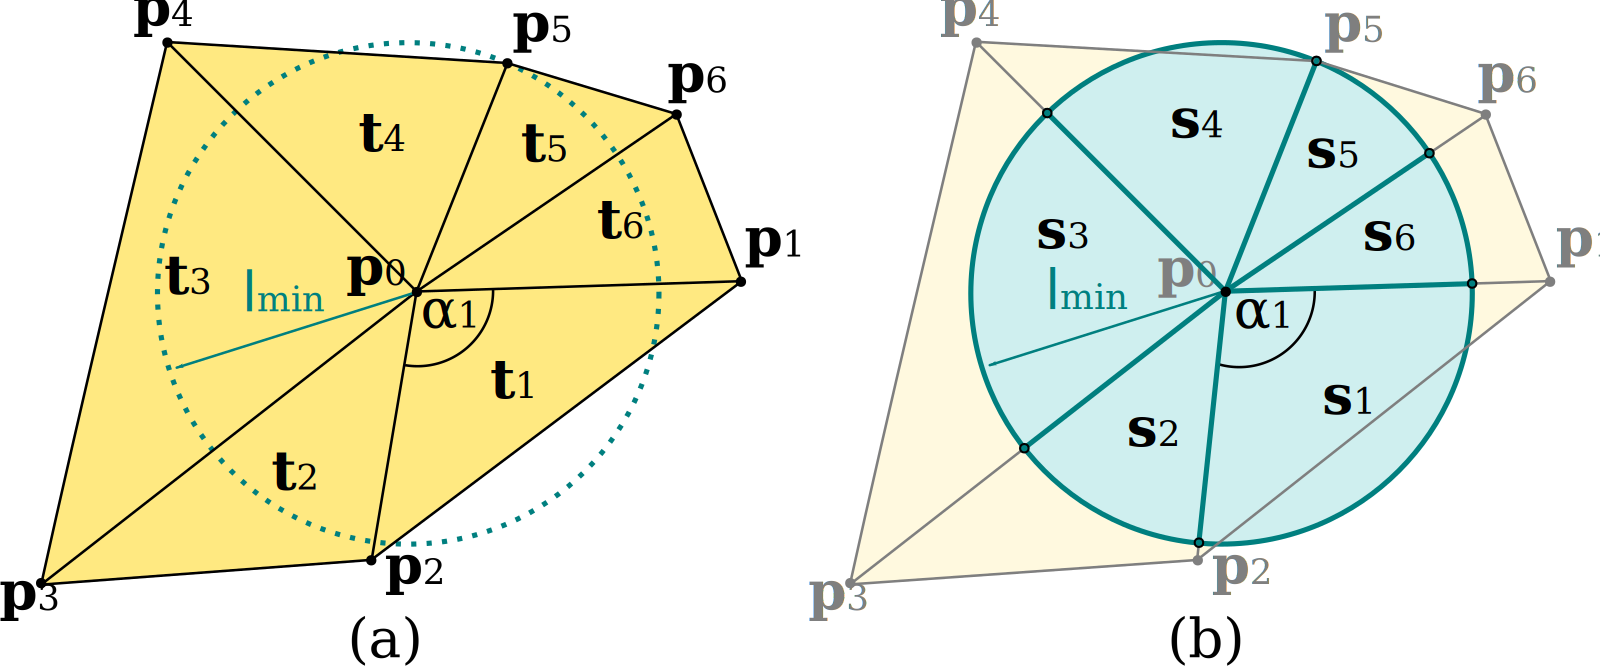
\includegraphics[width=1.0\linewidth]{figures/geodesicDisc.png}
	%\missingfigure{illustrate new geodesic disc algorithm idea}
	}{\caption[One-ring and geodesic disc]{A typical one-ring neighborhood $\mathcal{N}$ with (a) irregular triangular faces $\mathbf{t}_i$, the smallest edge length $\Dm = |\bp_4 - \bp_0|$ shown here with a cyan arrow as the radius of the geodesic disc, and $\alpha_1$ as the central angle of $\mathbf{t}_i$. (b) the complete geodesic disc, comprised of all its circular segments $\mathbf{s}_i$, each having central angles $\alpha_i$}\label{fig:geodesicDisc}}
\end{figure}%
\nomenclature{$\mathbf{s}_i$}{circular sectors which comprise the geodesic disc}

The function values $f'_i$ at the respective points $\bp_i$ along this disc are interpolated by 
\begin{equation}
	f'_i := f_0 + \Dm\frac{f_i-f_0}{|\bp_i-\bp_0|}
	\label{eq:avFuncValAtCoG}
\end{equation}

To calculate the weighted mean of the function value $\frac{\mathbf{f}'_i}{3}$ at each circle sector $\mathbf{s}_i$, we first compute
\begin{align}
	f^{\mathbf{s}}_i &:= f_0 + f'_i + f'_{i+1} \\
		& \: = 3f_0 + \Dm(\frac{f_i-f_0}{|\bp_i-\bp_0|} + \frac{f_{i+1}-f_0}{|\bp_{i+1}-\bp_0|}
	\label{eq:avFuncValAtCoG}
\end{align}
%
Next we compute average function value at the center of gravity of the circle sector
\begin{equation}
	f'_i := 
	%f_0 (1 - ( 2.0 * sin( alpha ) ) / ( 3.0 * alpha ) ) + ( funcValInterpolA + funcValInterpolB ) * ( 2.0 * sin( alpha ) ) / ( 3.0 * alpha ) / 2.0;
	\label{eq:avFuncValAtCoG}
\end{equation}
%
Finally, we can compute the one-ring weighted mean function value at $\bp_0$ as
\begin{equation}
	\bar{f}_0 := \frac{\sum A'_if^{\mathbf{s}}_i}{3A} \quad \forall i \in \{1,\ldots,n\}
	\label{eq:meanFuncValAtP0}
\end{equation}%
\nomenclature{$\bar{f}_0$}{the one-ring weighted mean function value at $\bp_0$}%

\bigskip
\bigskip
\bigskip
\bigskip
\bigskip
\bigskip
\bigskip
\bigskip

where $f_0$ is the function value of $\bp_0$. Note that $0 < \frac{
\Delta_\text{min}}{|\bp_i - \bp_0|} \leq 1$ such that the new 
$f'_i$ is always the weighted mean of $f_0$ and $f_i$ by the distance of the
respective points. For the weighted mean of the function value $\frac{f_i^t}{3}$ at 
each triangle $f^{\mathbf{t}'}_i$ we compute
\begin{align}
	f^{\mathbf{t}}_i & := f_0 + f'_i + f'_{i+1} \\
	& \: = 3f_0 + \Delta_\text{min}\left\lgroup\frac{f_i - f_0}{|\bp_i - \bp_0|} + 
	\frac{f_{i+1} - f_0}{|\bp_{i+1} - \bp_0|}\right\rgroup
\end{align}
So far we used the distance to the central point $\bp_0$ as weight 
function, but we also have to consider the distance of the points 
$\bp_i$ to their neighbors $\bp_{i+1}$ in the one-ring. We do this 
by computing the relative area of the geodesic disc marked by the three points 
$\bp_0$, $\bp_i$, and $\bp_{i+1}$. Instead of circle 
segments we approximate the geodesic disc by triangles $\mathbf{t}'_i$ achieving 
faster computation. As all those triangles are isosceles having two egdes of 
constant length $\Delta_\text{min}$ we can compute their weight as the area of the 
isosceles triangle $\mathbf{t}'_i$ using the Pythagorean theorem
\begin{equation}
	A'_i := |\mathbf{t}'_i| = \frac{|\bp_{i+1} - \bp_i|}{4}
	\sqrt{4\Delta_\text{min}^2 - |\bp_{i+1} - \bp_i|^2}
	\label{eq:areaFromPythagoreanTheorem}
\end{equation}
Regarding Figure~\ref{fig:geodesicDisc}a, the angle $\alpha_i$ could as well be 
used for weighting, computing $A'_i = \sin(\alpha_i)\Delta_text{min}^2$, which is 
equivalent to Equation~\ref{eq:areaFromPythagoreanTheorem}, but it 
is computationally expensive due to the $\sin(\cdot)$ operation and the numeric error 
is visible when the result of the mean filtering is rendered as color per 
vertex. Furthermore, computing $\Delta_\text{min}$ within each one-ring will cause 
tremendous amounts of redundant computing operations. Therefore we define 
\begin{equation}
	\overline{\Delta_\text{min}} := \min\{\Delta_\text{min}(\bp_0) | 
	\bp_0 \in \mathcal{M}\}
\end{equation} 
as the shortest edge for all triangles of the mesh. We will use this 
$\overline{\Delta_\text{min}}$ in all the above computations. This will increase the 
computing speed by a factor of $\approx 10$. 

For a one-ring we now compute the weighted mean function valuen with the total area
$A = \displaystyle\sum_{i=1}^nA'_i$ as
\begin{equation}
	\bar{f}_0 := \frac{\sum A'_if_i^\mathbf{t}}{3A} \quad \forall i \in \{1,\ldots,n\}
	\label{eq:weightedMean}
\end{equation}
with a negligible error due to the one-ring approximation of the geodesic 
disc.

For a one-ring weighted median filter instead, we can use all equations 
except~\ref{eq:weightedMean}, which is replaced by a list of pairs $(f_i^\mathbf{t}, 
A'_i)$ sorted by $f_i^\mathbf{t}$. The area is again used as a weight such that 
$1 = \displaystyle\sum_{j=1}^n\frac{A'_i}{A}$. The weighted median now becomes
\begin{equation}
\end{equation}
For the special case that $-$, which should not be excluded but rarely occurs, 
we compute $f  ̃ 0 =tf k t + f k+1$.~\cite[s.~3.2]{Mara17}



\section{GigaMesh}
The serial algorithm is not yet plublished, but was already implemented in Gigamesh.



\section{Summary}
Lorem ipsum dolor sit amet, consectetur adipiscing elit. Morbi tincidunt eget 
ipsum eu iaculis. Cras vel sem eu velit eleifend porta vel sit amet massa. Etiam 
a posuere nunc. Aenean aliquam viverra dapibus. Aliquam ac eros a purus feugiat 
rhoncus. Donec faucibus ut nibh ut cursus. Aliquam erat volutpat. Proin efficitur 
nulla sit amet iaculis condimentum. Cras placerat leo vitae venenatis feugiat. In 
hac habitasse platea dictumst. Orci varius natoque penatibus et magnis dis 
parturient montes, nascetur ridiculus mus. In aliquet sagittis dui eu pulvinar. 
Morbi a arcu eu dolor sagittis varius. Aliquam dignissim tortor sed tortor 
suscipit, eget imperdiet mauris convallis.
